\chapter{Problem analysis}
\section{State of the art} \label{sec:stateoftheart}
Stationary hover of drones is a subject with many known solutions, including quadcopters. Traditional quadcopters and other multirotor drones of similar design can obtain very high speeds, but consequently are quite ineffective with considerable power draws. Ineffective, meaning short flight times relative to the weight of the drone and its battery capacity. Drones from industry leaders such as DJI or Autel Drones typically have a flight time of approximately 30 minutes \cite{mavic2} \cite{MG-1} \cite{AutelEvo}.
The endgame for the proposed drone-design is an aircraft that can stay in the same location for long periods of time. With an efficient design, it should have low power usage with a small weight and great lift, resulting in much longer flight duration than traditional multirotor drone designs. 

\section{Previous work}
The drone used in this project is not an off-the-shelf product. Associate Professor Jens Christian Andersen made all the preliminary work and design choices.\\
The drone can be seen below in fig. \ref{fig:topviewdrone} and \ref{fig:bottomviewdrone}. A close-up of an arm can be seen in fig. \ref{fig:dronearmcloseup}.\\
At the beginning of the project period, the drone was equipped with some motors, custom PCB with sensors, microcontrollers, and a Raspberry Pi (RPi). A substantial amount of code had been written, especially for the microcontrollers and some for the Raspberry Pi, though the drone did not function at the time. 
The drone body is made from 3D printed plastic. As much as possible of this work will be reused.\\
\begin{figure}[h!]
    \centering
    \begin{minipage}[t]{.48\textwidth}
        \centering
        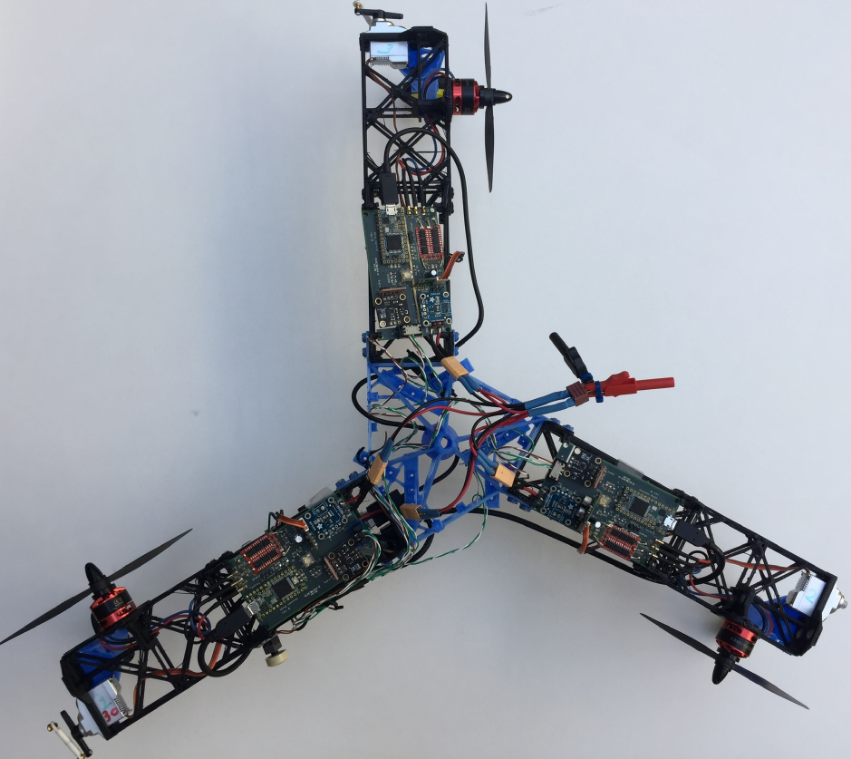
\includegraphics[width=0.93\textwidth]{figures/analysis/overview.png}
        \caption{Overview of the drone. Notice each arm has one propeller motor, one wing tilt servo motor and one module with sensors etc}
        \label{fig:topviewdrone}
    \end{minipage}%
    \hspace{.03\textwidth}
    \begin{minipage}[t]{0.48\textwidth}
        \centering
        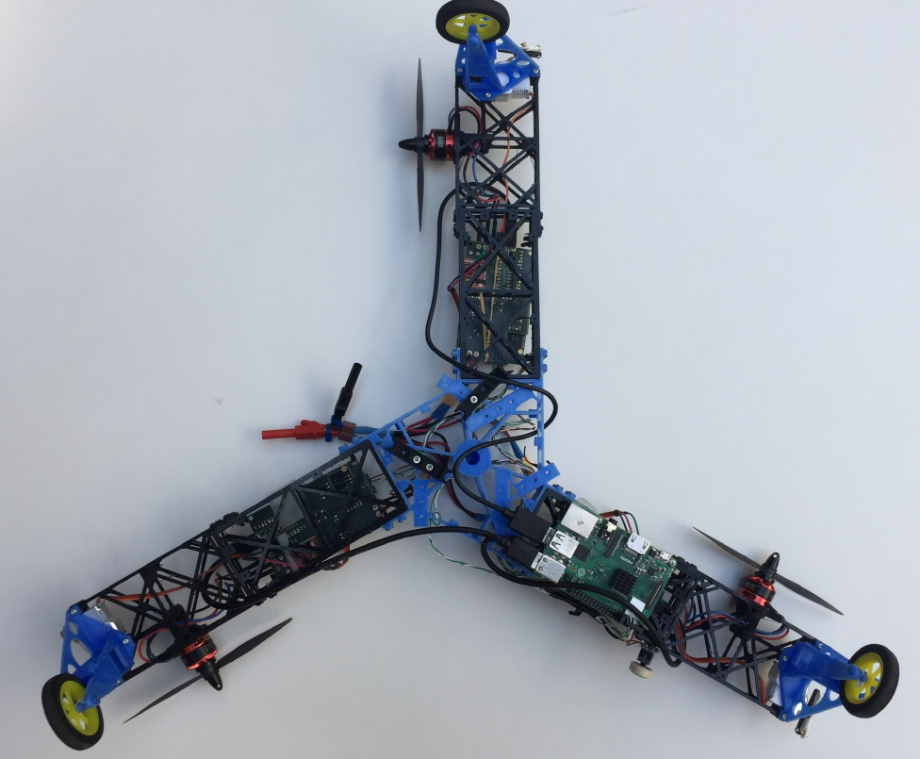
\includegraphics[width=1\textwidth]{figures/analysis/bottomview.png}
        \caption{Bottom view of the drone. Notice the Raspberry Pi, and lack of batteries}
        \label{fig:bottomviewdrone}
    \end{minipage}
\end{figure} 

\begin{figure}[h!]
    \centering
    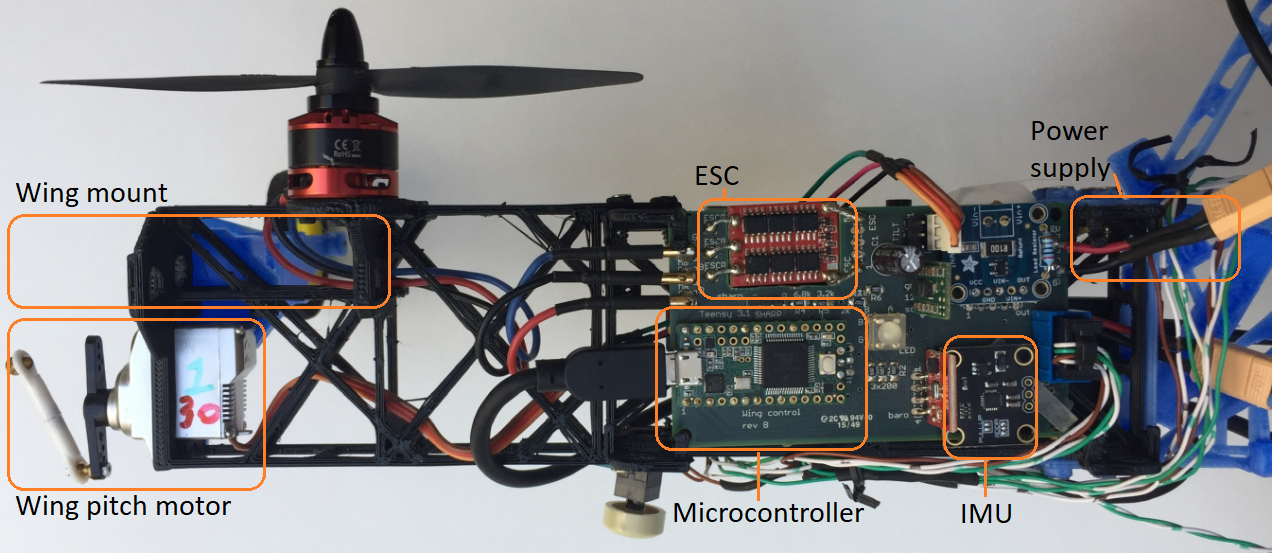
\includegraphics[width=0.9\textwidth]{figures/analysis/arm_closeup.png}
    \caption{Close up view of one drone arm}
    \label{fig:dronearmcloseup}
\end{figure}
The following subsections elaborate upon the details of the drone.

\subsection{Motors}
There are two types of motors on the drone: the propeller motor, which creates forward thrust to spin the drone in a circular motion, and the wing tilt motor that controls the tilt of the wing. \\
The propeller motor is a 2300 kV brushless DC motor for 3S and 4S battery configurations \cite{propellermotordata}, which means that the motor needs a battery with 3 or 4 cells in series to have sufficient voltage to run. The kV rating suggests it will approximately run 2300 RPM per volt across the motor with no load.  \\
The wing tilt motor is a 3 Blue Bird BMS 380 Max servo motor, and can be configured from 4.8V to 6V \cite{tiltmotor}. Continuous PWM-signals control it. The motor is quite capable -- at 6V it has a torque of 4.7 $kg\cdot cm$. 

\subsection{Modules} 
Each of the drone's three arms consists of a printed circuit board (PCB) with multiple sensors, a few small circuits, and a microcontroller. 
The components are:
\begin{itemize}
    \item A Teensy microcontroller version 3.2 \cite{teensy32}.
    \item An MPU-9250; a 9-DoF inertial measurement unit (IMU) with accelerometer, gyroscope, and magnetometer. \cite{mpu-9250}.
    \item A BMP180 barometric pressure, temperature, and altitude sensor \cite{BMP180}.
    \item An INA169 analog current sensor breakout board using the INA169 current shunt monitor from Burr-Brown \cite{INA169}.
    \item A 10A UBEC electronic speed control that uses Li-Po batteries \cite{HK10AESC}.
    \item An RGB LED
    \item A D24V22F6, which is a 6V, 2.5A Step-Down Voltage Regulator from Pololu \cite{PololuStepDown}.
    \item Supporting circuitry, input- and output pins for power and data transmission.
\end{itemize}
The converter steps down the voltage from the batteries to 6V usable by the wing tilt motor. The ESC controls the propeller motor. Barometer, MPU-9250, and INA169 are used to obtain data about the drone and its state. The microcontroller ties everything together.
%and facilitates the communication between arm and Raspberry Pi. 

\subsection{Microcontroller}
A Teensy 3.2 microcontroller is used to monitor and control all that happens on each arm. The Teensy's goal is to receive sensor data and communicate with the CPU. The microcontroller also streamlines the received data into easy-to-read formats (SI-units) for both the CPU and user.

\subsection{CPU} %
The drone's CPU is a Raspberry Pi (RPi) 3B+. It is responsible for centralizing data from all three arms and the processing of it. The processed data establish the changes to the propeller motor's RPM and the servo motor's position for each arm. As such, the RPi transmits commands that invoke the necessary changes. 

\section{Analysis of objectives}\label{analysisofgoals}
For the drone to control its rotational speed relative to a reference point, some hardware work must be done. It is necessary to have a fully functioning hardware setup before any other work can start. Due to the nature of this project, much work must go into this, as it is a physical prototype of this new design. \\
Reliable communication between microcontrollers and the RPi is crucial because otherwise, no data transfer or calculation can be made. When this is complete, the sensor usage can begin, and it should then be possible to start analyzing the data in real-time to gain information about the orientation and state of the drone.  \\
In the end, a control loop can be implemented either in a simulation using a model or on the prototype, with the goal of stabilizing the rotational speed in reference to a set point. \\
An in-depth analysis of what specifically needs to be done can be seen in the next five subsections.


\subsection{Hardware design}\label{hardwaregoals}
Three main goals have to be completed:
\begin{enumerate}
    \item Constructing a suitable battery pack that has the correct specifications and an appropriate capacity. The capacity has to be high enough to endure long flight times, but also not too heavy for efficient flight. 
    \item Programming the microcontroller so that all sensors are usable, and both the propeller and wing tilt motor can be controlled. Functions for sending and receiving data are needed as well.
    \item Choosing wings of an appropriate design and mounting them. Wing types and designs have to be analyzed, and an appropriate way to fit them is needed. They have to be mounted both on the drone body, and to the wing tilt motor so the pitch can be controlled. 
\end{enumerate}
These goals will be explored in chapter \ref{chap:comm_hardware}. 

\subsection{Communication}\label{commgoals}
The primary objective is to design easy to use and "fast enough" communication between the microcontrollers and RPi, relative to the needed update frequency of the control loop. A concurrent programming solution will be considered.
This goal will be explored in chapter \ref{chap:comm_hardware}.

\subsection{Sensor data and usage}\label{sensorgoals}
For sensor data, two main objectives have to be achieved:
\begin{enumerate}
    \item Stable outputs of sensors that result in good measurements and usable data. 
    \item Combining sensor data to gain knowledge about roll, pitch, and yaw, as well as where the drone is in its rotation and its orientation relative to true north. 
\end{enumerate}
These goals will be explored in chapter \ref{chap:sensordataandusage}.

\subsection{Control loop}\label{controlloopgoals}
A well-functioning control loop has to be implemented. A good loop will hopefully result in fast, and stable performance, that lets the drone react to small irregularities as well as significant changes. This loop will have one key objective: to control the rotational velocity of the drone. A PD-controller with a feed-forward branch will be examined in chapter \ref{controlloopchapter}.


\subsection{System modelling}\label{modelgoals}
The system will be simplified and modeled using Matlab and Simulink for gathering and analyzing comparable data. Additionally, the model will be used for preliminary testing of the drone's capabilities and its controller.
This goal will be explored further in chapter \ref{chap:systemmodelling}, and implemented in section \ref{results:rotcontroller}. 